\section{ДУ в полных дифференциалах}
\begin{Def}
    ДУ вида
    \[
        M(x,\;y)\,dx+N(x,\;y)\,dy=0 \qquad M(x,\;y),\; N(x,\;y)\in C'(D)
    \] 
    называется ДУ <<в полных дифференциалах>>, если $\exists F(x,\;y) \in C^{\textcolor{red}{2}}(D)$ для которой
    \begin{gather*}
        F'_x=M(x,\;y)\\
        F'_y=N(x,\;y)
    \end{gather*}
    то есть ДУ имеет вид $dF(x,\;y)=0$\\
    
    \textcolor{cyan}{Примечание.} Дифференциал \[dF(x,\;y)=F'_x\,dx+F'_y\, dy=M\,dx+N\,dy\] является полным, поэтому и название уравнения <<в полных дифференциалах>>.
\end{Def}

\begin{Th}[Об общем интеграле]
    В условиях определения 1, уравнение $F(x,\;y) = C$ даёт общий интеграл ДУ $dF(x,\;y)=0$ (предполагаем, что D-односвязная область (ограниченная простой замкнутой кривой))
\end{Th}

\begin{Proof}
    Интегральная кривая $dF(x,\, y) = 0$
    \begin{gather*}
        L:
        \begin{cases}
            x=x(t)\\
            y=y(t) 
        \end{cases} \quad t\in I\\
        \Leftrightarrow\\
        \exists C = const, \quad \forall t \in I, \quad F(x(t),\, y(t))= C
    \end{gather*}
    \begin{enumerate}
        \item[\textcolor{blue}{$\Rightarrow$}]
        По условию имеем
        \[
            F_x'(x(t),\,y(t))\,x'_t+F_y'(x(t),\,y(t))\,y'_t=0
        \]
        Значит
        \begin{align*}
            &(F(x(t),y(t)))'=0, \quad t \in I\\
            \Rightarrow \; &\exists C = const \quad \forall t \in I \quad F(x(t),\, y(t)) = C
        \end{align*}
        
        \item[\textcolor{blue}{$\Leftarrow$}] По условию 
        \[
            \forall t \in I \quad F(x(t),\, y(t))= C
        \]
        Продиференцируем равенство, получим
        \[
            F_x'\,x'_t + F_y'\,y'_t = 0
        \]
        По определению следует, что\\
        $L$ --- интегральная кривая ДУ $F_x'\,dy+F_y'\,dx = 0$ и значит $dF(x,y)=0$
    \end{enumerate}
\end{Proof}

\begin{Note}[решение задачи Коши]
    \[
        \begin{cases}
            dF(x,y)=0\\
            y|_{x=x_0}=y_0
        \end{cases}
    \]
    $F(x,y)=F(x_0,y_0)$ (в неявном виде)\\
\end{Note}

\begin{Example}
    Дано
    \[
        F(x,y)=x^2\,y 
    \]
    Требуется вывести ДУ.\\
    Решение.
    \begin{align*}
        F'_x &=2\,x\,y\\
        F'_y &= x^2
    \end{align*}
    Тогда уравнение <<в полных диференциалах>> будет выглядеть так
    \begin{floatingfigure}[l]{50mm}
        \noindent
        \hfil
        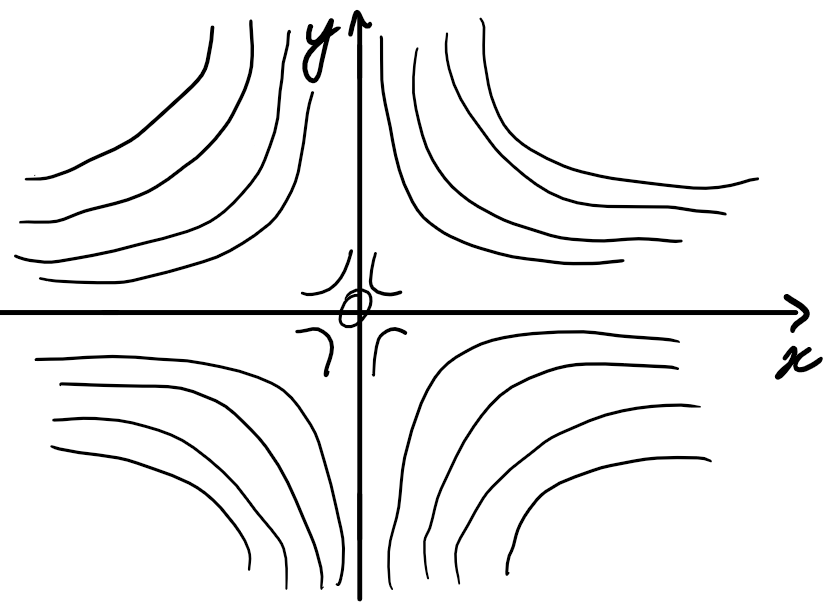
\includegraphics[width=45mm]{pictures/2_5_1.png}
        \caption{Общее решение}
        \hfil
    \end{floatingfigure}
    \begin{gather*}
        2\,x\,y\,dx+x^2\,dy = 0\\
        x^2\,y + x^2\,y = C_1\\
        x^2\,y = C = \frac{C_1}{2}
    \end{gather*}
    Общее решение
    \[
        y=\frac{C}{x^2}
    \]
\end{Example}

\begin{Th}[О необходимом и достаточных усл. хар. ДУ в полн. диф.]
    Пусть функции $M(x,\; y) \quad N(x,\; y) \in C'(D)$, где $D$ односвязная замкнутая ограниченная область на $\bb{R}^2$ (граница $D$ односвязанная замкнутая кривая). Тогда ДУ 
    \[
        M(x,\; y)dx + N(x,\; y)dy = 0
    \] 
    является ДУ в полных дифференциалах. Это эквивалентно 
    \[
        M'_y = N'_x \qquad (\forall(x,\; y) \in \mathring{U}(D))
    \]
\end{Th}

\begin{Proof}
    Пусть $M_0(x_0, y_0)$ - внутренняя точка в области D
    \begin{enumerate}
        \item[\textcolor{blue}{$\Rightarrow$}]
            Пусть есть $F(x,y)\in C^{\textcolor{red}{2}}$ такая, что 
            \[
                F'_x=M(x,\,y), \quad F'_y=N(x,\,y) \quad \forall (x,y) \in \mathring{D}
            \]
            \begin{figure}[bh]
                \noindent\centering{
                    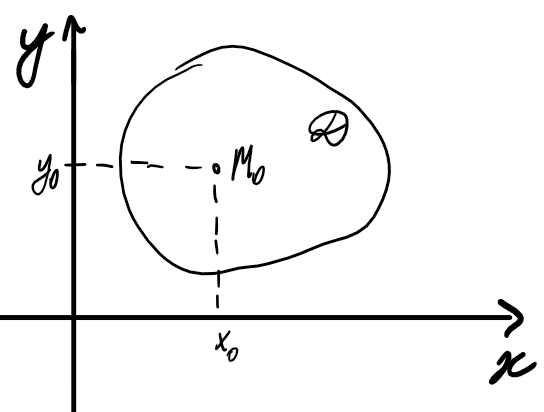
\includegraphics[width=45mm]{pictures/2_5_2.png}
                    \caption{}
                }
            \end{figure}
            Найдём $M'_y=F''_{xy}\in \mathring{D}\in C(\mathring{D})$ и $N'_x=F''_{yx}\in C(\mathring{D})$\\
            Так как они непрерывны, значит $F''_{xy}=F''_{yx}$. Из этого очевидно, что 
            \[
                 M'_y=N'_x \qquad M'_y, N'_x \in \mathring{D}
            \]
        
        \item[\textcolor{blue}{$\Leftarrow$}] По условию
            \[
                \forall (x,y) \in \overset{\circ}{D} \quad M'_y(x,y)=N'_x(x,y)
            \]
            и возьмём
            \[
                (x_0,\; y_0) \in \mathring{D}, \quad U((x_0,\; y_0)) \subset D
            \]
            Найдём частный интеграл $F'_x$, где $y=const$
            \[
                F'_x=M(x,y) \quad \Rightarrow \quad F(x,\,y)=\int_{x_0}^{x}M(x;\,y)\,dx+\varphi(y)
            \]
            Также
            \begin{gather*}
                F'_y=\left(\int_{x_0}^{x}M(x,\;y)\,dx+\varphi(y)\right)'_y=\int_{x_0}^{x}M'_y(x,\;y)\,dx + \varphi'(y) \equiv N(x,\;y)\\
                \int_{x_0}^{x}N'_x(x,\; y)\,dx = N(x,\; y)\\
                \int_{x_0}^{x}N'(x,y)\,dx+\varphi'(y) \equiv N(x,y)\\
                N(x,y)|_{x_0}^x + \varphi' \equiv N(x,y)\\
                \cancel{N(x,y)} - N(x_0,y) + \varphi'_y \equiv \cancel{N(x,y)}\\
                \varphi'_y=N(x_0,y)\\
                \varphi(y)=\int_{y_0}^{y}N(x_0, y)\,dy
            \end{gather*}
            Таким образом
            \[
                F(x,y)=\int_{x_0}^{x}M(t,y)\,dt+\int_{y_0}^{y}N(x_0,s)ds
            \]
            
            \textcolor{cyan}{Замечание.} По поводу односвязанности.\\
            Односвязность показывает то, что мы способны соединить точки $P$ и $P_0$ внутри данной области.\\
            \begin{figure}[h!]
                \noindent\centering{
                    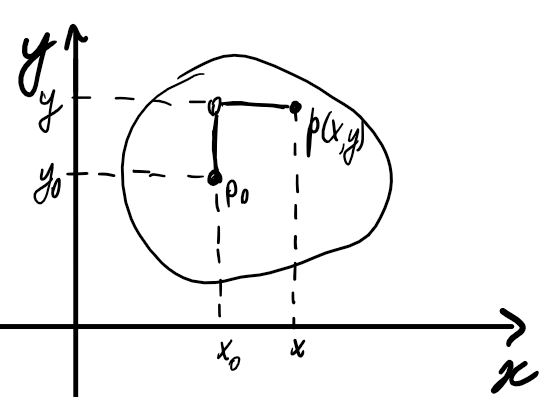
\includegraphics[width=45mm]{pictures/2_5_3.png}
                    \caption{}
                }
            \end{figure}
            Тогда $\exists F(x,y)$ определённая в $U(P_0)$
            \begin{equation*}
                F'_x=M(x,y) \quad F'_y=N(x,y) \qquad (\forall (x,y) \in U(P_0))
            \end{equation*}
            <<Двигаем>> точку $P_0$ до $P$. Тогда\\
            \pagebreak
            \begin{figure}[h!]
                \noindent\centering{
                    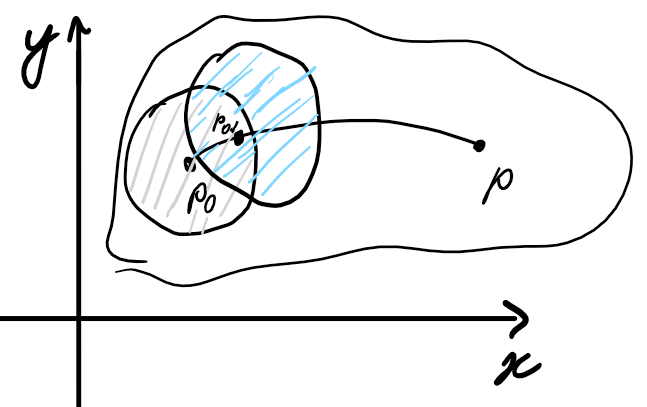
\includegraphics[width=45mm]{pictures/2_5_4.png}
                    \caption{<<движение точки>>}
                }
            \end{figure}
            \[
                \exists F(x,y) \in \mathring{D} \qquad  F'_x=M \qquad F'_y=N \quad (\forall (x,y) \in \mathring{D})
            \]
    \end{enumerate}
\end{Proof}

\begin{Def}[Интегрирующий множитель]
    Пусть 
    \[
        M(x,y),\; N(x,y) \in C'(D)
    \]
    Тогда функцию $\mu = \mu(x,\;y)$ называют интегрирующим множителем ДУ
    \[
        M\,dx + N\,dy=0
    \]
    Или (\textcolor{cyan}{$\Leftrightarrow$})\\
    Существует $\mu(x,\;y)$ --- непрерывная функция, причём ДУ\\
    \[
        \mu\,M\,dx+ \mu\,N\,dy = 0
    \] 
    является ДУ <<в полных дифференциалах>>.\\
    Или
    \[
        u(x,\;y) \in C'(D) \qquad (\mu\,M)'_y=(\mu\,N)'_x
    \]
    в односвязных компонентах области $D$ и частях $D$
\end{Def}


\begin{Note}(отыскание интегрирующего множителя в некоторых случаях)\\
    \begin{enumerate}
    	\item 
    Пусть 
    \[
        \frac{M'_y-N'_x}{N}=f(x)
    \]
    Тогда существует интегрирующий множитель
    \[
        \mu=\mu(x) \qquad \mu(x)=e^{\int f(x)dx}
    \]
    \item А если  
    \[
	    \frac{M'_y-N'_x}{M}=g(y)
    \]
    Тогда существует интегрирующий множитель
    \[
    \mu=\mu(y) \qquad \mu(y)=e^{-\int g(y)dy}
    \]
    \end{enumerate}
\end{Note}  

\begin{Proof}
    \begin{enumerate}
    	\item Рассмотрим
    	\begin{gather*}
    	    \mu'_y\,M+\mu\,M'_y=\mu'_x\,N+\mu\,N'_x\\
    	    \mu\,(M'_y-N'_x)=\mu'_x\,N-\mu'_y\,M\\
    	\end{gather*}
    	Если $\mu = \mu(x) \quad \mu'_y \equiv 0$, тогда
    	\begin{gather*}
    	    \frac{d\mu}{\mu}=\frac{M'_y-N'_x}{N}\,dx=f(x)\,dx\\
    	    \ln|\mu|=\int f(x)\,dx\\
    	    \mu(x)=e^{\int f(x)\,dx}\\
    	\end{gather*}
    	\item Если
    	\[
    	\mu = \mu(y) \Rightarrow \mu'_x \equiv 0\]
    	тогда 
    	\[
    	\frac{d\mu}{\mu} = -\frac{M'_y-N'_x}{M}\,dy=-g(y)\,dy\]
    	\[
    	\mu(y)=e^{-\int g(y)\,dy}\\
    	\]
    \end{enumerate}
\end{Proof}

\begin{Example}
    Дано
    \[
        x\,y\,dx+(x^2+y^2)\,dy=0
    \]
    Решение
    \begin{align*}
        M&=xy & N&=x^2+y^2\\
        M'_y&=x & N'_y&=2x
    \end{align*}
    \[
        \frac{M'_y-N'_x}{M}=-\frac{x}{x\,y}=-\frac{1}{y}=g(y)
    \]
    Из замечания выше следует
    \begin{align*}  
        \exists \mu=\mu(y)=e^{\int g(y)dy}=e^{\int \frac{dy}{y}}=e^{\ln y}&=y\\
        \mu&=y
    \end{align*}
    Таким образом $y=\mu$. Домножим равенство из условия на $y$.
    \begin{gather*} 
        x\,y^2\,dx+(x^2y+y^3)\,dy=0\\
        M_1=xy^2\\
        N_1=x^2y+y^3\\
        M'_{1_y}=2\,x\,y=N'_{1_x}\\
    \end{gather*}
    Таким образом получили ДУ в полных диференциалах.\\
    Решаем его
    \begin{gather*} 
        \begin{cases}
            F'_x=xy^2\\
            F'_y=x^2y+y^3
        \end{cases}
    \end{gather*}
    Возьмём первое уравнение и проинтегрируем его. Причём вместо константы добавим функцию от $y$ (можем т.к. $(\varphi(y))'_x = C'_x = 0$).
    \begin{gather*} 
        F(x,\,y) = \int x\,y^2\,dx=y^2\int x\,dx=\frac{y^2 x^2}{2}+\varphi(y)
    \end{gather*}
    Найдём $\varphi(y)$ с помощью $F'_y$
    \begin{gather*} 
        (\frac{1}{2}x^2y^2+\varphi(y))'_y=x^2y+y^3\\
        x^2y+\varphi'_y=x^2y+y^3\\
        \varphi'_y=y^3 \quad \varphi(y)=\frac{y^4}{4}
    \end{gather*}
    Таким образом мы нашли $F(x,\;y)$. Ответом является следующее уравнение
    \begin{equation*}
        \frac{1}{2}x^2y^2+\frac{1}{4}y^4 = C
    \end{equation*}
\end{Example}
